\chapter{Implementation details}
\label{cha:implementation}

Software engineering decisions, problems/solutions and resignations will be discussed in this chapter.

\section{Software engineering decisions}

\subsection{Why to re-implement the calibration estimation package?}

Willow Garage has an already implemented calibration package:

\url{http://www.ros.org/wiki/calibration}

\noindent
It is a more generic package, it is able to calibrate joint angles and different type of sensors all together.
My code is a github fork of this repository:

\url{https://github.com/pablospe/calibration}

\noindent
Then, why to re-implement it? A number of points: % was desired: % and the original package does not has:
\begin{itemize*}
 \item Difficult to support new robot models.
 \item Poor performance.
 \item Implemented in Python. Rewrite in C++ was required in order to use Ceres Solver, KDL and URDF C++ parser.
 \item The old calibration package uses DH parameters\footnote{The Denavit-Hartenberg parameters (DH parameters) are the four parameters associated with a particular convention for attaching reference frames to the links of a spatial kinematic chain, or robot manipulator.}, which has some problems with certain robots.
\end{itemize*}

Mainly for these points, the estimation was decided to be rewritten from scratch.



\subsection{Why KDL?}

As mentioned above, the old package uses DH parameters and it has its own kinematic library, instead of using the well tested KDL. Besides forward kinematic, KDL was useful for geometric frame transformations and conversion between quaternions and angle-axis (rotation matrix parameterization).



\subsection{Why to re-implement \texttt{robot\_state\_publisher}?}

\texttt{robot\_state\_publisher} is a package in ROS which publishes the state of a robot to \texttt{/tf}. It takes the joint angles of the robot as input and publishes the 3D poses of the robot links, using a kinematic tree model of the robot (KDL tree which is obtained from the URDF description).

There are two problems with this package:
\begin{itemize*}
 \item It does not allow to modify the URDF without constructing a new \texttt{robot\_state\_publisher} from the tree model. Note the importance of this because the main goal of calibration is to update the URDF. In addition, since it is an optimization process and it must be as fast as possible, it was not desired to send/receive messages during this stage.

 \item Another problem is that the fixed joints (non-mobile joints) are published half a second later (for some unknown reason), and when the URDF is updated strange behavior might occur.
\end{itemize*}

%
% Why KDL? KDL structures are not modificable, so it was needed to re-create KDL once the urdf is updated.
%
% RViz and Markers! Republish everytime!
%
% * Quaternions: used to avoid singularities...
%
% * Data/Views in different order... explain... some views aren't visible for all the cameras.
%
% (optional)
% Why Ceres?

\subsection{Quaternions}

One important observation is the use of quaternions. This decision was taken to avoid singularities that others rotation parameterization may have.

\newpage
\section{Code}
\subsection{Cost function}
\label{sec:ceres_impl}

The Ceres Solver cost function implemented is simple, mainly because distortion is not needed to be considered, since the images are already rectified.

\begin{lstlisting}[language=C++, label=code:cost_function, caption={Cost function}]
template <typename T>
void calc_residuals(double observed_x, double observed_y,
                    double fx, double fy, double cx, double cy,
                    const T* const camera_rotation,
                    const T* const camera_translation,
                    const T* const point,
                    T residuals[2])
{
  // camera_rotation are the quaternions
  T p[3];
  ceres::QuaternionRotatePoint(camera_rotation, point, p);

  // camera_translation is the translation
  p[0] += camera_translation[0];
  p[1] += camera_translation[1];
  p[2] += camera_translation[2];

  // Compute the projection
  T xp = p[0] / p[2];
  T yp = p[1] / p[2];
  T predicted_x = T(fx) * xp + T(cx);
  T predicted_y = T(fy) * yp + T(cy);

  // The error is the difference between the predicted and observed position.
  residuals[0] = predicted_x - T(observed_x);
  residuals[1] = predicted_y - T(observed_y);
}
\end{lstlisting}



\subsection{N-View Triangulation}
\label{sec:triangulation_impl}

This is a generalization of the triangulation method proposed in section \ref{sec:triangulation}.

\begin{lstlisting}[language=C++, label=code:triangulation, caption={Triangulation}]
// It is the standard DLT (for multiple views)
void nViewTriangulate(const Mat_<double> &x,
                      const vector<Matx34d> &Ps,
                      Vec3d &X)
{
  unsigned nviews = x.cols;

  CV_Assert(x.rows == 2);
  CV_Assert(nviews == Ps.size());

  Mat_<double> design = Mat_<double>::zeros(2 * nviews, 4);
  for (int i = 0; i < nviews; ++i) {
    for (int j = 0; j < 4; ++j) {
      design(i*2,   j) = x(0,i) * Ps[i](2, j) - Ps[i](0, j);
      design(i*2+1, j) = x(1,i) * Ps[i](2, j) - Ps[i](1, j);
    }
  }

  Mat X_homog;
  cv::SVD::solveZ(design, X_homog);
  homogeneousToEuclidean(X_homog, X);
}
\end{lstlisting}

% \section{...}

% \subsection{Creating model point for solvePnP}
% \label{sec:solvePnP_impl}
% It is was necessary to create a function that
%
% \begin{lstlisting}[language=C++, label=code:generateCorners, caption={generateCorners}]
% void ChessBoard::generateCorners(vector<Point3d> *corners)
% {
%   // clear corners
%   corners->clear();
%
%   // generate corners: (x,y,z)
%   for ( int j = 0; j < height_; j++ )
%     for ( int i = 0; i < width_; i++ )
%       corners->push_back( Point3d( float(i*square_size_),
%                                    float(j*square_size_), 0 ) );
% }
% \end{lstlisting}


\section{Problems and solutions}

\subsection{Visible cameras}

\textbf{Problem}: depending of the point of view, not all the checkerboards are visible by all the cameras (see Figure \ref{fig:visibility}). Moreover, the order of the cameras in the ROS messages can change. This complicated the whole process adding unexpected complexity to simple tasks. It could have been avoided with a better design in the acquisition part.

\begin{figure}[!htbp]
 \centering
 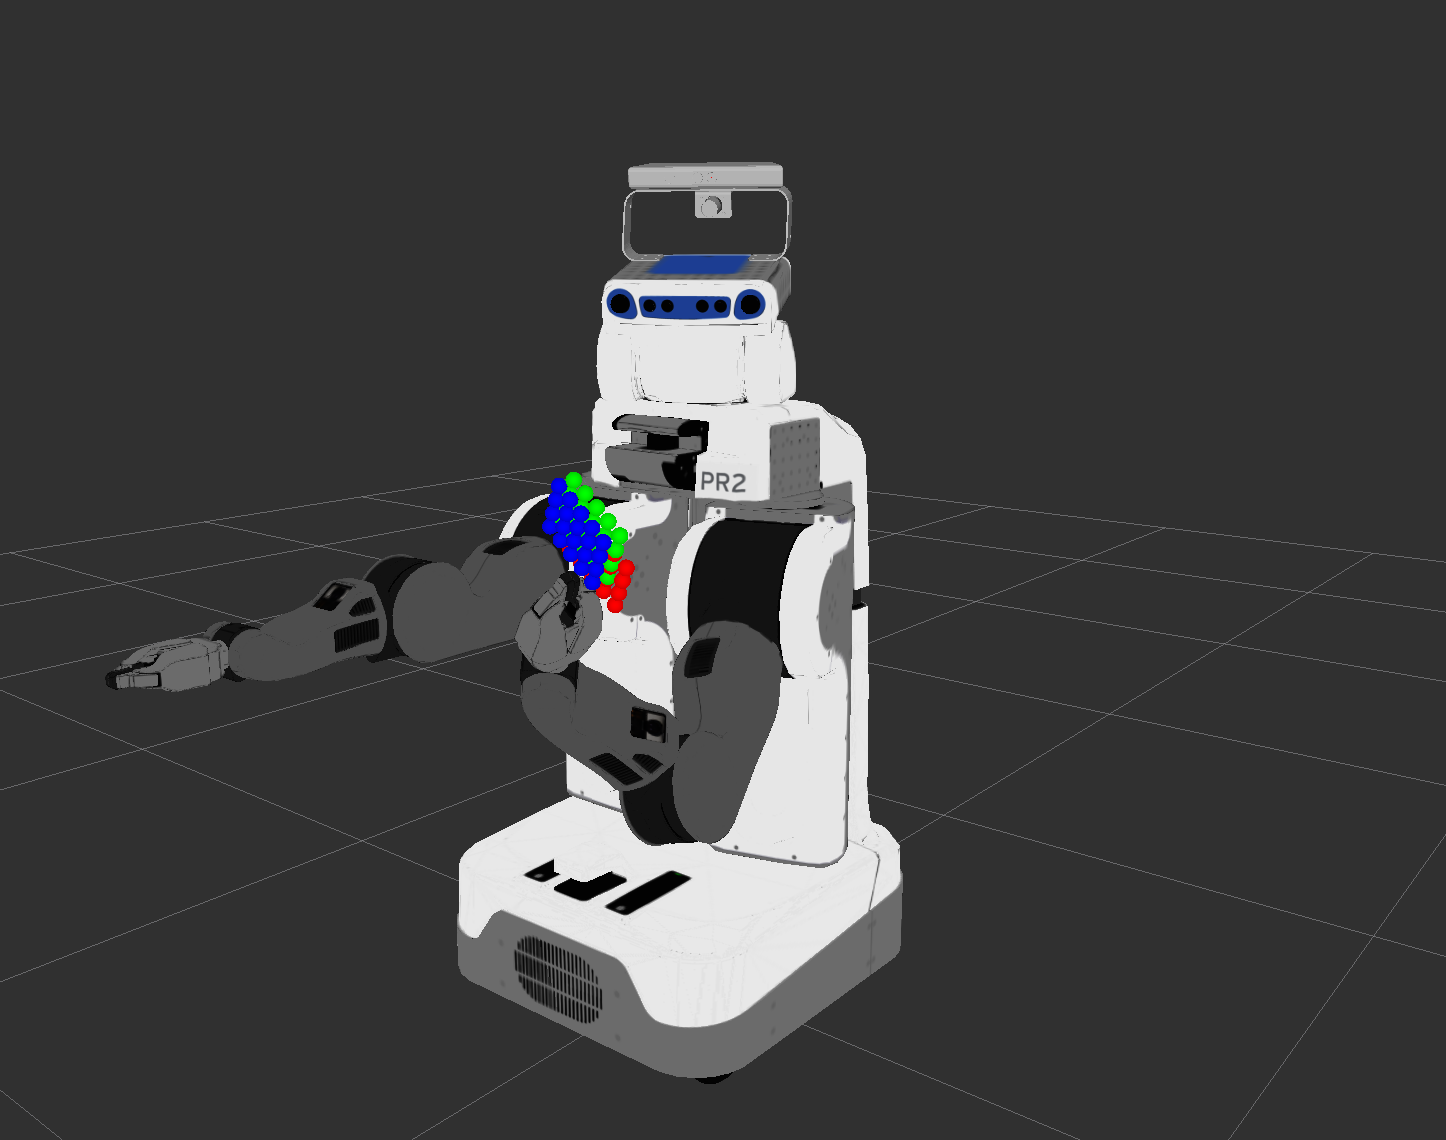
\includegraphics[width=0.65\textwidth]{images/screenshots/uncalib05.png}
 \caption{Checkerboard in hand visible only for 3 cameras.}
 \label{fig:visibility}
\end{figure}

\noindent
\textbf{Solution}: A class called \texttt{View} was created which works as a data container with a well defined camera order. It has some ``mapping'' between cameras and frame names (coordinate system names).

\subsection{Visual Markers}

\textbf{Problem}: if the number of checkerboard is reduced (less cameras can see the checkerboard), old markers will remain in the scene.

\noindent
\textbf{Solution}: erasing all markers and publishing periodically with a timer.

\subsection{Robot update}

\textbf{Problem}: once the optimization process finishes, the result is not ready to be use. The rotation and translation matrices are relative to the first camera, and cannot be used to update the robot. A example in Figure \ref{fig:optimization_failer}, which was one of the initial ``solutions''.

\noindent
\textbf{Solution}: an explanation of how to update the robot after the optimization process is given in section \ref{sec:update_urdf}.

\begin{figure}[!htbp]
 \centering
 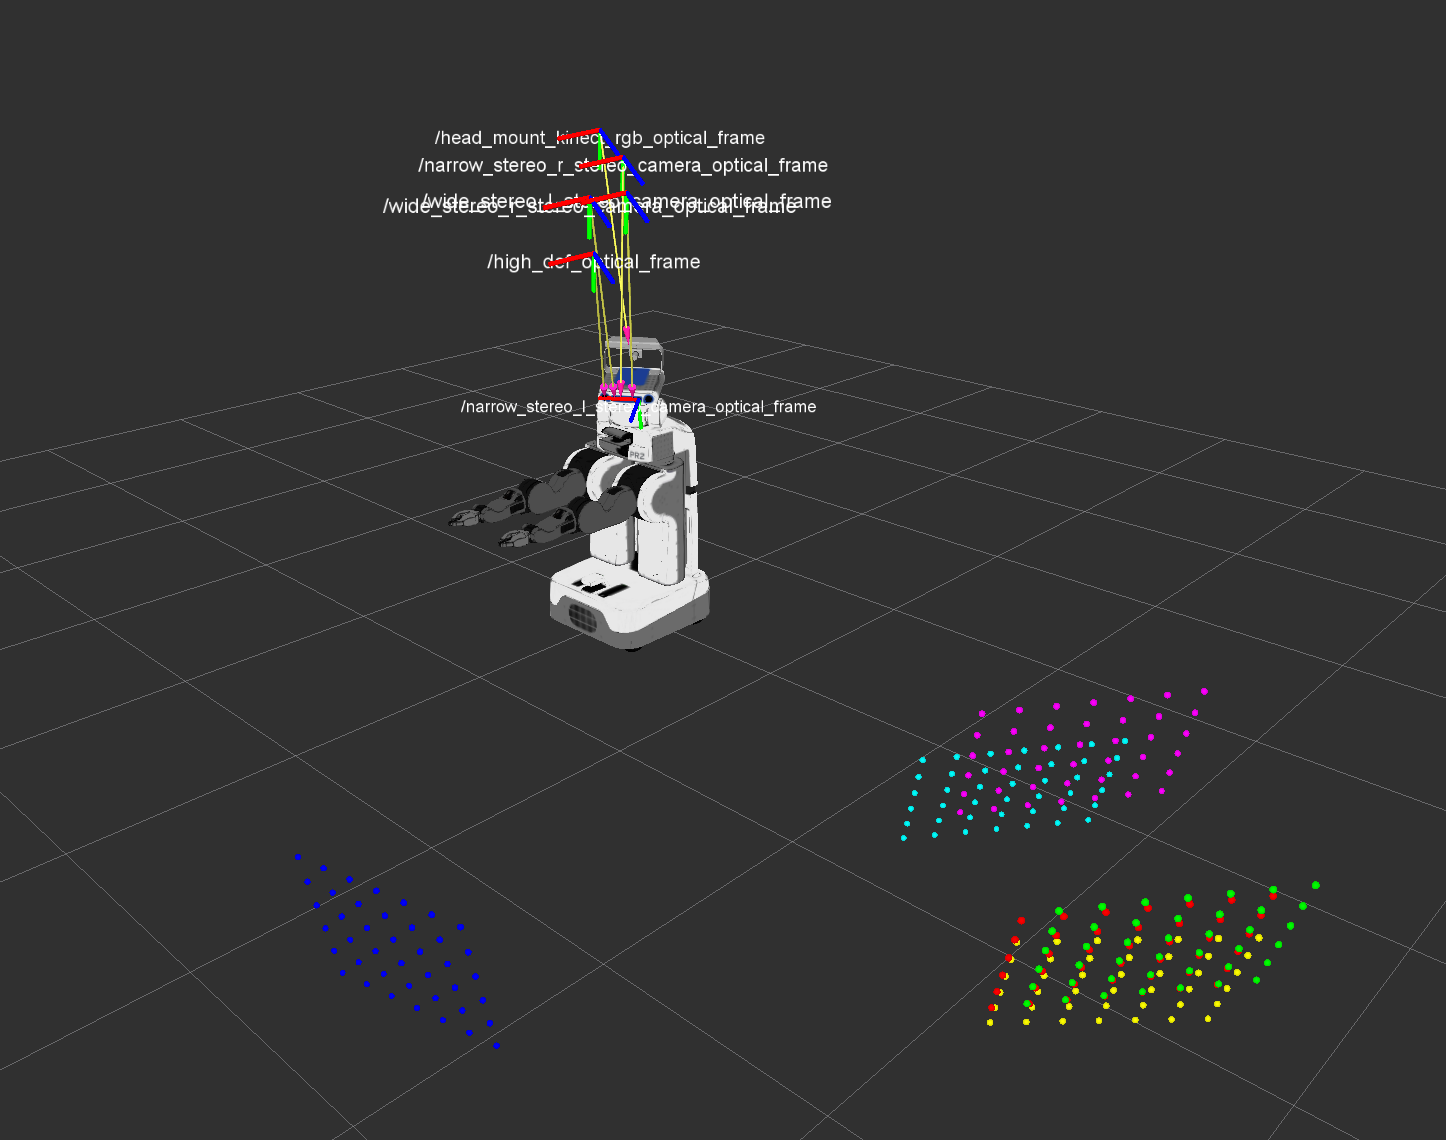
\includegraphics[width=0.6\textwidth]{images/screenshots/optimization_failer02_2.png}
 \caption{Initial versions}
 \label{fig:optimization_failer}
\end{figure}


\newpage
\subsection{Multi-view triangulation}

\textbf{Problem}: multi-view triangulation method is not as precise as expected, see Figure \ref{fig:triangulation_fails}.

\noindent
\textbf{Solution}: more analysis is required to find why the reprojection error is large.

\begin{figure}[!htbp]
 \centering
 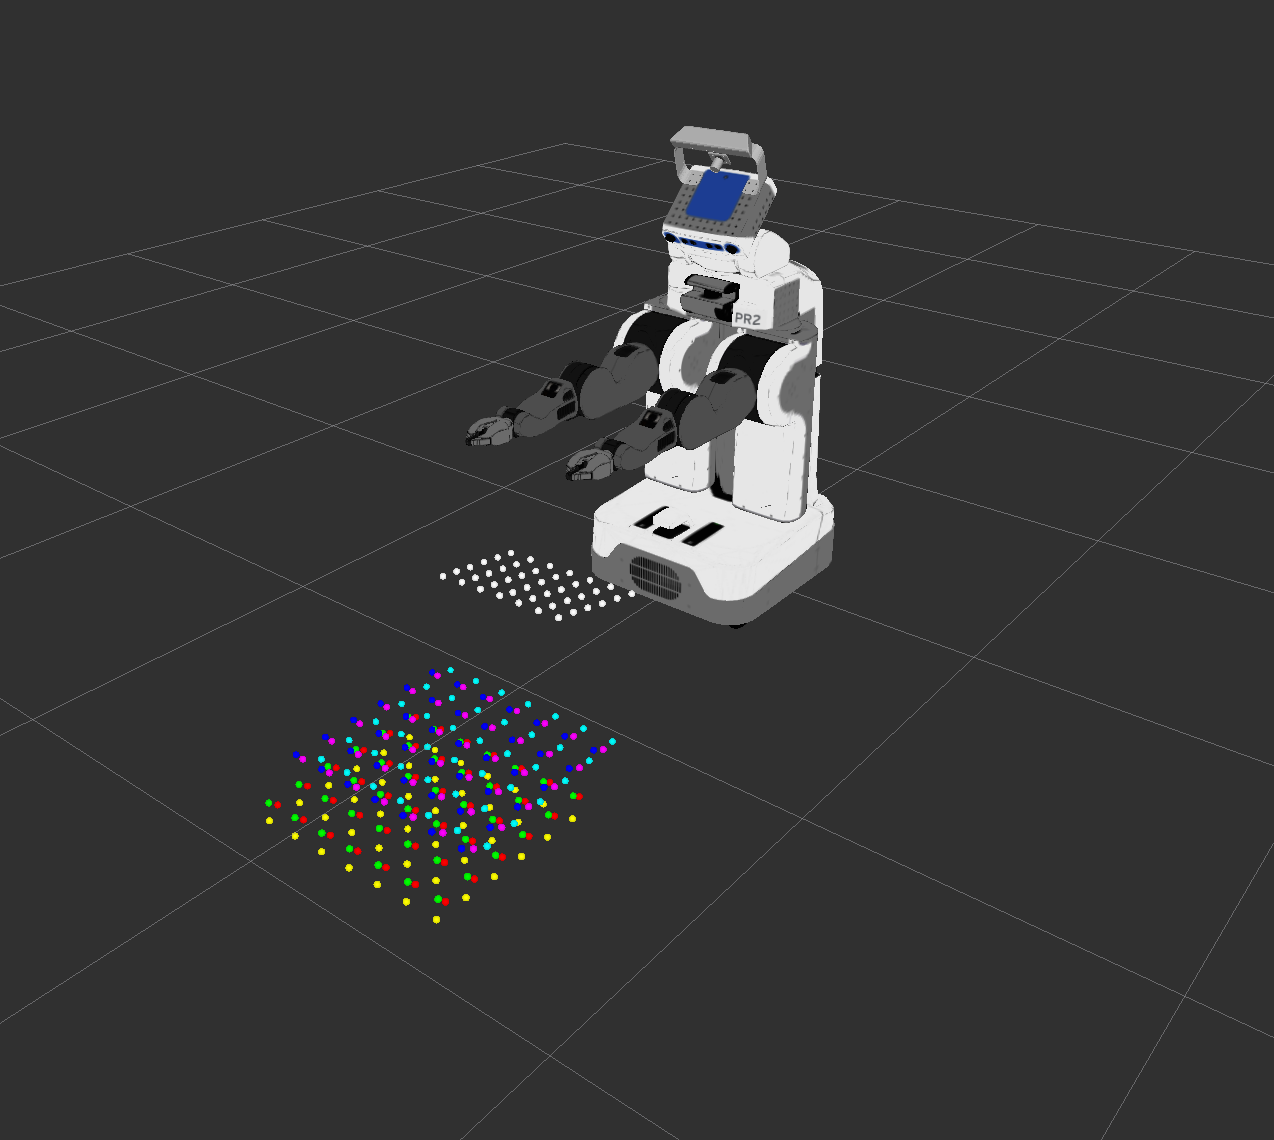
\includegraphics[width=0.6\textwidth]{images/screenshots/triangulation_fails.png}
 \caption{Triangulation points (white dots) must be closer to solvePnP solutions (color dots)}
 \label{fig:triangulation_fails}
\end{figure}

\vspace*{-2ex}
\section{Stats}
Just for fun, it took me 9,061 additions and 3,954 deletions in 99 commits until this point.
\begin{figure}[!htbp]
 \centering
 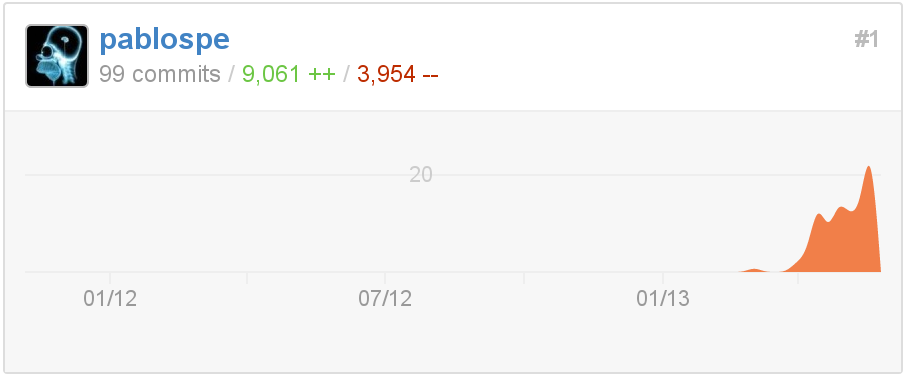
\includegraphics[width=0.65\textwidth]{images/git_stats.png}
 \caption{Github stats}
 \label{fig:git_stats}
\end{figure}

Github repository: \url{https://github.com/pablospe/calibration}.

% \chapter{Extra work}
% \label{cha:extra}
%
% (this chapter is more than optional)
%
% Work not related to the thesis, but time consuming, like commits in Ceres, fixed bugs in URDF dom (export\_urdf() function), etc...

